\cotefile{45}
\scanpage{18}
% source line 1; boxed heading
\noindent\fbox{Borel \unsure{est} son propre normalisateur}

% source lines 2--5
\diagram{\begin{tikzcd}[ampersand replacement=\&,column sep=small]
\text{(i) }\underline{B}\text{ normalisateur de }\unsure{\mathscr L|\mathcal L}\arrow[rr,Leftrightarrow]
\& {} \& \text{(ii) }\mathscr L\text{ normalisateur de }\mathscr L \\
\& \text{(iii)}\arrow[u,Leftrightarrow] \& {}
\end{tikzcd}}
\diagram{\begin{tikzcd}[ampersand replacement=\&]
\operatorname{Drap}(G)\arrow[r]\arrow[d,equal]\arrow[dr]
\& \operatorname{Grass}(\unsure{\mathfrak g|\mathscr G})\arrow[d,phantom,"\cup" description]\quad\unsure{imm} \\
G/B \& G/\operatorname{Norm}_{G}(\mathscr L)
\end{tikzcd}}
\noindent\unsure{par} $g\mapsto\operatorname{int}(g).B$

% source line 6
$(\mathrm i)\Rightarrow(\mathrm{ii})$ trivial, car $\operatorname{Lie}N_{\unsure{G}}(\unsure{B|\mathscr L})=\operatorname{Norm}_{\mathfrak g}\mathscr L$

% source lines 7--10
$(\mathrm{ii})\Rightarrow(\mathrm i)$, car soit $B'$ le normalisateur, $B'\supset B$, il \unsure{a} $\unsure{=|\text{même}}$ algèbre de Lie alors $B=B'{}^0$, donc $B'$ normalise $B$ \unsure{ensemblist\textsuperscript{t}}, donc $B\unsure{\subset|=}B'$ \unsure{ensemblist\textsuperscript{t}}, donc $B=B'$

% source lines 11--19; the large outlined block is crossed out throughout.
$(\mathrm{ii})\Leftrightarrow(\mathrm{iii})$, \inserted{trivial}
\deleted{\unsure{en} \unsure{prenant} les \unsure{différentielles} \unsure{sur} les \unsure{espaces} \unsure{localisés} en $B$ resp $\mathscr L$, \unsure{on} \unsure{trouve}}
\diagram{\begin{tikzcd}[ampersand replacement=\&]
\deleted{\mathfrak g/\mathscr L}\arrow[r]\arrow[dr]
\& \deleted{\operatorname{Grass}(\mathfrak g)}\arrow[d,phantom,"\deleted{\cup}" description]\quad\deleted{\text{(}\unsure{\text{espace tangent}}\text{)}} \\
{} \& \deleted{\operatorname{Hom}(\mathscr L,\mathfrak g/\mathscr L)}
\end{tikzcd}}
\deleted{\unsure{par} $\dot x\mapsto\unsure{\mathfrak g|\varphi}D_x(\mathscr L)$, \unsure{qui} \unsure{est} \unsure{d'où} \unsure{le} \unsure{noyau} $\unsure{\to|=}\operatorname{Norm}_{\mathfrak g}(\mathscr L)/\mathscr L$. Donc $(\mathrm{ii})$ signifie que $\operatorname{Drap}(G)\to\operatorname{Grass}(\mathfrak g)$ \unsure{est} \uline{non ramifié}, \deleted{\unsure{donc}} il en résulte que \unsure{c'est} \unsure{une} \unsure{imm}, car le normalisateur de}

% source lines 20--21
Ces conditions ne sont pas tjrs vérifiées, \unsure{p.ex.} $\operatorname{SL}(2)$ en car $2$ les met en défaut.
% archive sheet number: 17
\scanpage{19}
% source lines 1--4; diagonal cancellation through this draft.
\deleted{\uline{Corollaire.} Dans le cas où $K\subset G$ \inserted{\unsure{de ss schéma fermé}}, $G$ de t. multiplicatif de t.f. sur $S$, [$\exists\unsure{n}$ \unsure{tel|tq} \unsure{que|pour} $K\subset{}_{\unsure{n}}G$, or ${}_{n}G$ est fini sur $S$] $K$ est fini sur $S$.}
% source lines 5--7
\deleted{Donc si \unsure{la|1|sa} \unsure{fibre} en un p\textsuperscript{t} est \unsure{réduit|réduite} au corps résiduel kif kif \unsure{aux} p\textsuperscript{ts} voisins par Nakayama !}

\medskip\noindent\rule{1.6cm}{0.4pt}
% isolated rightward stroke below the separator
\[\unsure{\longrightarrow}\]

% source lines 8--10
\deleted{Rem : prouver le lemme sur \unsure{tt|les} \unsure{sous-grpe|sous-grpes} d'un diagonalisable sur un corps. On utilise le}

% source lines 11--16
\deleted{\uline{Lemme de Chevalley}. Soit $G$ grpe affine \inserted{de t. fini} sur $k$, $H$ ss-grp de $G$. Alors $\exists$ repr. linéaire de $G$ sur un $V$, et un $x\in V^*$, tel que $H$ soit le stabilisateur de $\bar x$ dans la \unsure{repr.} projective \unsure{correspondante}.}
% archive sheet number: 18
\scanpage{20}
% source lines 1--2
\[
\begin{aligned}
1)\quad &B\text{ normalisateur de }\unsure{\mathscr L|\mathcal L}\Longleftrightarrow\mathscr L\text{ normalisateur de }\mathscr L\\
&\Longleftrightarrow(\operatorname{Drap}(G)\longrightarrow\operatorname{Grass}(\unsure{\mathfrak g|\mathscr G}))\text{ monomorphisme}
\end{aligned}
\]
% source lines 3--4
faux en général pour $G$ \unsure{demi-simple|semi-simple} \unsure{non} \unsure{adjoint} (exemple $\unsure{\operatorname{SL}|\operatorname{GL}}(2,k)$, $k$ de car $2$)

% source line 5
\deleted{\unsure{2)} $B$ connu quand on connaît $\mathscr L$}

% source lines 6--8
\[
1')\quad\operatorname{Drap}(G)\longrightarrow\operatorname{Grass}(\mathfrak g)\quad\text{injectif ??}
\]
\margin{\uline{\unsure{tjrs|tjs} radiciel}}
% slanted
C'est vrai pour $G=\unsure{\operatorname{PSL}|\operatorname{SL}}(2)\deleted{\unsure{k}}$, mais moins intéressant car ce n'est pas un monomorphisme

% source lines 9--11; the insertion is circled, as is the displayed map.
\usetikzlibrary{shapes.geometric}
2) $T\subset G$ \inserted{\mbox{\tikz[baseline=(c.base)]{\node[draw,ellipse,inner sep=1pt] (c) {tore maximal};}}} donné, $\operatorname{Drap}_{T}(G)$ schéma des Borels cont\textsuperscript{t} $T$, est-il vrai que
\diagram{\begin{tikzcd}[ampersand replacement=\&]
|[draw,ellipse]| \operatorname{Drap}_{T}(G)\longrightarrow\operatorname{Grass}(\mathfrak g)\quad\text{est un \uline{monomorphisme}?}
\end{tikzcd}}
% source lines 12--14
\deleted{Comme} Il suffit (comme $\operatorname{Drap}_{T}(G)$ est étale sur $k$) que ce soit géom. \uline{injectif}. à fortiori, que $\operatorname{Drap}(G)\to\operatorname{Grass}(\mathfrak g)$ le soit

% source lines 15--19
\deleted{Or, si $B\supset T$} On est ramené au cas $G$ \unsure{demi-simple|semi-simple}, et dans ce cas on sait que $B$ est \deleted{engendré par} $T.\prod_{\alpha\in\unsure{\Phi|\varphi}}P_\alpha$, où \deleted{les $P_\alpha$} \inserted{les} \deleted{\unsure{aux} \unsure{racines}} $P_\alpha$ \unsure{grpes} \unsure{radiciels} \deleted{sont les} \unsure{correspondant} aux $\mathfrak g_\alpha\unsure{\subset|\in}\mathscr L$, donc déterminés par $\unsure{B|\mathscr L}$.
% archive sheet number: 19
\scanpage{21}
% source lines 1--8; draft cancelled with long diagonal strokes.
\deleted{\uline{Théorème} $G$ comme dessus, $C$ un sous-grpe de Cartan, $H$ un sous-schéma en groupes de $G$, simple$/S$, à fibres connexes, \uline{contenant $C$}, $\unsure{\mathfrak h|\mathscr H}\subset\unsure{\mathfrak g|\mathscr G}$ \unsure{algèbre} de Lie. Alors $H$ est déterminé de façon unique par $C$ et $\mathfrak h$ et les conditions précédentes, i.e. $\forall$ autre ss-grpe $H_1$ \unsure{satisfaisant} aux ces conditions et tel que $\mathfrak h_1=\mathfrak h$, est égal à $H$.}

% source line 9; locally struck opening within the cancelled draft.
\deleted{Lorsque les} \deleted{Soit $T$ le tore maximal de $C$.}

% source lines 10--15
\deleted{Lorsque les caractères infinitésimaux [\unsure{pour} \unsure{sur} $\unsure{\mathfrak t|t}=\operatorname{Lie}(T)$] de $T$ opérant sur $\mathfrak g/\mathfrak h$ sont $\ne0$ sur chaque fibre, de sorte que sur chaque fibre $\mathfrak h$ est son propre normalisateur, alors par Exposé de Demazure, il s'ensuit que $H=\operatorname{Norm}_{G}(\mathfrak h)^{\unsure{0|\circ}}$, et on gagne.}

% source lines 16--21
\deleted{Dans le cas général, soit $\unsure{\mathfrak z|Z}$ le centre \unsure{réductif} de $G$, qui est $\subset T$, donc dans $H$. \unsure{Ceci dit|Quitte à} : \unsure{diviser|divisant} par $\mathfrak z$, on} \deleted{\unsure{donc}} \deleted{est ramené à la situation où $\mathfrak z=0$. Alors $\mathfrak t$ opère \uline{fidèlement}}
% archive sheet number: 20
\scanpage{22}
\usetikzlibrary{shapes.geometric}
% source lines 1--4
3) $G$ schéma en groupes réductif sur $S$, $B$ sous-schéma en groupes \unsure{simple|lisse}$/S$ induisant sur chaque fibre un Borel. Est-ce que $B$ est un Borel ?? / Oui, car on se ramène au cas semi-simple adjoint\unsure{....}

% source lines 5--9; outlined argument cancelled diagonally.
\deleted{\unsure{Par descente|Par dessus|Pour démontrer}, on peut supposer que $B$ contient un tore maximal de $G$ \inserted{\mbox{\tikz[baseline=(c.base)]{\node[draw,ellipse,inner sep=1pt] (c) {déployé};}}}. Alors $\unsure{\mathscr L|\mathcal L}=\unsure{\mathfrak t|t}+\sum_{\alpha\in\unsure{P|\Phi}}\unsure{\mathfrak g|\mathscr G}_\alpha$, \unsure{le|où} $P$ un ``ens de racines positives''. Donc il existe un Borel $B'$ ayant même $\mathscr L$.}

% source lines 10--14
Laissons tomber l'hypothèse $G$ réductif,

\deleted{On peut \unsure{espérer} \unsure{par} \unsure{dessus} que} on se demande si deux tels $B,B'$ sont \inserted{\unsure{loc\textsuperscript{t}|loc}} \uline{conjugués} \deleted{par extension \unsure{fid\textsuperscript{t}}} \inserted{au sens de la top.} \unsure{fidèl\textsuperscript{t}|fid\textsuperscript{t}} plate quasi \unsure{cpte|cpt}. Cela se \unsure{ramène|vérifie} sur les fibres géométriques : la question
% source line 15
\[
H^{\unsure{1}}(\unsure{B|\mathscr L},\mathfrak g/\mathscr L)=0\qquad??
\]
% source line 16
du point \uline{de vue infinitésimal}.

% source lines 17--19
On peut supposer que $B$ et $B'$ contiennent un $=$ tore $T$, et [\deleted{\unsure{de}} \unsure{quitte} au voisinage du point $s\in S$] que $B_s=B'_s$
% archive sheet number: 21
\scanpage{23}
% source lines 1--7; entire theorem draft crossed diagonally.
\deleted{\uline{Théorème} (?) $\unsure{G|C}$ grpe affine simple$/k$. Soit $\bar k$ clôture algébrique, $\bar G=G_{\bar k}$, $\bar T$ un tore maximal de $\bar G$,}
\deleted{\unsure{supposons}}
\deleted{$\bar R$ le radical de $\bar G$,}
\deleted{On considère \unsure{supposons} que les}
\deleted{$\unsure{\overline{\mathfrak r}|\overline{\mathscr R}}\subset\unsure{\overline{\mathfrak g}|\overline{\mathscr G}}$ les algèbres de Lie, on suppose que les ``racines'' \inserted{non nulles,} de $\bar T$ intervenant dans $\overline{\mathfrak g}/\overline{\mathfrak r}$ n'interviennent pas dans $\overline{\mathfrak r}$}
\deleted{[\unsure{p.ce.|p.ex.} que $\overline{\mathfrak r}$}
\deleted{\inserted{[p.ex. que $\bar T$ opère trivialement sur $\overline{\mathfrak r}_{u}$]} Alors $\bar R$ est défini sur $k$.}
% archive sheet number: 22
\scanpage{24}
\usetikzlibrary{shapes.geometric}
% Upright layer, from the upper edge downwards. Several diagonal cancellations
% intersect writing in a second orientation; their extent is uncertain.
\[G=\unsure{\operatorname{Aff}|\operatorname{GP}}(\unsure{G_a|\mathfrak g})\]
\[
\deleted{\operatorname{Hom}_{\unsure{k'\text{-alg}|k'\otimes_k k'}}(\unsure{k'},G)=G'}
\]
\diagram{\begin{tikzcd}[ampersand replacement=\&]
\deleted{G}\arrow[r]\&\deleted{G'}\arrow[r]\&{}\&\deleted{\unsure{\mathscr L|\mathcal L}}
\end{tikzcd}}
\deleted{\uline{\unsure{ss-grpe} \unsure{invariant}}}
\[\deleted{R_1\subset G_1}\qquad\unsure{\mathfrak h|h}\]
\diagram{\begin{tikzcd}[ampersand replacement=\&,row sep=small]
k_0(t^{\unsure{1/p|1/q}})\arrow[d,dash]\\
k_0(t)
\end{tikzcd}}
\[\unsure{h_1|k_1}\]
\diagram{\begin{tikzcd}[ampersand replacement=\&,column sep=large]
{}\arrow[rr,leftrightarrow,bend left=20]\&\deleted{\unsure{\mathfrak g|\mathscr G}}\ G\&{}
\end{tikzcd}}
\diagram{\begin{tikzcd}[ampersand replacement=\&]
\deleted{G}\arrow[r,bend left=10]\&\deleted{G'}\arrow[l,bend left=35,"\deleted{\unsure{\operatorname{Norm}_{k'/k}}}"']\&R'\&\deleted{B}
\end{tikzcd}}
\[G\qquad\mathfrak g\quad\unsure{\mathfrak h|h}\qquad H^1\]
\[\boxed{\deleted{\mathfrak g\quad\mathfrak g}}\]
% The unlabelled double-cone/hourglass drawing between the two boxed equalities.
\figure{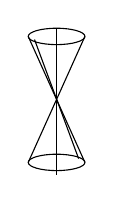
\begin{tikzpicture}[x=0.8cm,y=0.8cm]
\draw (0,2) ellipse (0.45 and 0.13);
\draw (-0.45,2)--(0.45,0) (0.45,2)--(-0.45,0);
\draw (0,0) ellipse (0.45 and 0.13);
\draw (0,2.13)--(0,-0.2);
\draw (-0.35,1.95)--(0.35,0.06);
\end{tikzpicture}}
\diagram{\begin{tikzcd}[ampersand replacement=\&]
\deleted{\mathscr L,=\mathscr L'}\&
\boxed{\deleted{[B_0=B'_0]\quad B,B'\supset T}}\arrow[d,Rightarrow,"?"']\\
{}\&\deleted{\unsure{B|R}=B'}
\end{tikzcd}}
\noindent En car $\ne\text{\uuline{$2,3,5$}}$

O.K.
\[\boxed{\deleted{\mathscr L=\mathscr L'}}\qquad\deleted{\unsure{R|B}}\]
\[H^1(B,\mathscr L)\]

% Left-edge layer, read clockwise through 90 degrees. Shared labels occur once.
% margin note written sideways; its arrows connect to the adjacent statements.
\diagram{\begin{tikzcd}[ampersand replacement=\&,column sep=small,row sep=large]
{}\&\begin{gathered}\text{Radical \inserted{\mbox{\tikz[baseline=(c.base)]{\node[draw,ellipse,inner sep=1pt] (c) {\unsure{géométrique|géométr.}};}}} défini sur }k,\\
\text{pour tt \unsure{grpe} sur tt corps }k\end{gathered}\\
\deleted{\unsure{H^1(B,\mathfrak g/\mathfrak b)=0}}\arrow[r,Rightarrow,bend left=15]\&
\begin{gathered}\text{Une \uline{variation infinitésimale}}\quad\inserted{\mbox{\tikz[baseline=(c.base)]{\node[draw,ellipse,inner sep=1pt] (c) {$\unsure{k'/k|\bar k/k}$};}}}\\
\text{d'un \uline{Borel} est \uline{triviale}}\\
\text{(i.e. }\unsure{\bar k|k'}\text{\unsure{-conjugué})}\end{gathered}\arrow[u,Rightarrow]\arrow[d,Leftrightarrow]\\
\unsure{H^1(\mathfrak u,\mathfrak u)^{T}=0|H^1(u,u)^T=0}\arrow[u,Rightarrow]\&
\begin{gathered}\text{\uline{Une telle variation}, avec un tore maximal fixé,}\\
G\text{ est \uline{constant}.}\end{gathered}
\end{tikzcd}}
% margin note written sideways; upper part of the narrow inner column
\margin{($R$ radical \uline{\unsure{unip.}}) \illegible{2}}
\[
H^1(R,\deleted{\unsure{\mathfrak g}}\mathfrak g/\mathscr L)^{B/R}=0
\]
\diagram{\begin{tikzcd}[ampersand replacement=\&,column sep=small]
{}\arrow[r]\&\deleted{H^1(B',\mathfrak g/\mathscr L)}\arrow[r]\&
\deleted{H^1(B,\mathfrak g/\mathscr L)}\arrow[r]\&
\deleted{\underline{H^1(\unsure{k'/k|k'},\mathfrak g/\mathscr L)^{B'}}}
\end{tikzcd}}
% Right-edge note, also read clockwise.
% margin note written sideways
\margin{Ça se déforme dans $G.\mathfrak g$ \deleted{$\operatorname{SL}(2).\unsure{\mathfrak{sl}(2)|\operatorname{sl}(2)}$} pour $G=\operatorname{SL}(2)$ (\uline{$\unsure{H_e|H}$} \unsure{anti-algèbre|cohomologique|pathologique}).}
% Lower-right boxed note, read clockwise. The end is crossed by an arrow.
% margin note written sideways
\margin{\fbox{\parbox{1.8cm}{il suffit que les \unsure{caractères} de $T$ \unsure{intervenant|intervenants} dans $\mathfrak g/\mathscr L$ n'interviennent pas \unsure{dans} \illegible{1}}}}
% Isolated broad arrow at the bottom-left corner.
\figure{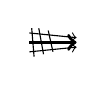
\begin{tikzpicture}[x=0.3cm,y=0.3cm]
\draw[->,line width=1.2pt] (0,0)--(2,0);
\draw[->] (0,0.4)--(2,0.2);
\draw[->] (0,-0.4)--(2,-0.2);
\draw (0.2,-0.6)--(0.1,0.6) (0.6,-0.5)--(0.4,0.6) (1,-0.4)--(0.8,0.5);
\end{tikzpicture}}
% archive sheet number: 23
\scanpage{25}
\usetikzlibrary{shapes.geometric}
% archive sheet number: 24
% Whole draft cancelled by two long diagonal strokes.
\margin{\mbox{\tikz[baseline=(c.base)]{\node[draw,ellipse,inner sep=1pt] (c) {\deleted{\unsure{$G$ comme dessus}}};}}}

% Source lines 1--7.
\deleted{\uline{Théorème} Soit $H$ un sous-grpe de $G$, simple/$S$ et à fibres connexes, ayant $\unsure{=|\text{même}}$ rang réductif et $=$ \unsure{rg|rang} \unsure{unipotent|unip.} que $G$, \deleted{Alors} \deleted{\unsure{$H$ est le}} \unsure{soit} $\unsure{\mathfrak h|\mathscr H}=\operatorname{Lie}(H)\subset\unsure{\mathfrak g|\mathscr G}=\operatorname{Lie}(G)$. \deleted{Alors} Alors $H$ est le \uline{normalisateur connexe} de $\mathfrak h$ dans $G$ \deleted{\unsure{(qui a le rg}} (opérant sur $\mathfrak g$ par la représentation adjointe).}

% Source lines 8--16.
\deleted{En effet, Demazure a montré qu'il suffit de prouver que pour tt fibre géométrique, le normalisateur de $\mathfrak h$ dans \uuline{$\mathfrak g$} est égal à $\mathfrak h$. On peut donc supposer $S$ spectre d'un corps alg. clos, et \deleted{\unsure{on a}} \unsure{notre|not.} hypothèse signifie alors que $H$ contient un sous-groupe de Cartan $C$ \uline{de $G$} ; soit $T$ \unsure{son|un} tore maximal.}
\scanpage{26}
% archive sheet number: 25
% Source lines 1--2.
\uline{Théorème} $G$ \unsure{schéma} en groupes affine connexe sur $k$, $B$ Borel, $\unsure{\mathscr L|\mathcal L}\subset\unsure{\mathfrak g|\mathscr G}$ alg. de Lie. Alors
\[
B=\operatorname{Norm}_{G}(B)\tag*{a)}
\]
\margin{? ---}
\[
\begin{aligned}
B&\longrightarrow\operatorname{Norm}_{G}(\mathscr L)\quad\text{est \uline{surjectif}, donc}\\
\operatorname{Drap}(G)&\longrightarrow\operatorname{Grass}(\mathfrak g)\quad\text{injectif (pas tjrs une imm.)}
\end{aligned}
\tag*{b)}
\]

% Source lines 6--9; an earlier item letter is struck above c).
\deleted{\unsure{c)|b)}} c) Conditions équivalentes
\[
\begin{aligned}
\text{i)}\quad B&=\operatorname{Norm}_{G}(\mathscr L)
&\text{ii)}\quad\mathscr L&=\operatorname{Norm}_{\mathfrak g}(\mathscr L)\\
\text{iii)}\quad\operatorname{Drap}(G)&\longrightarrow\operatorname{Grass}(\mathfrak g)\quad\text{une imm.}
\end{aligned}
\]
\smallskip\hrule\smallskip
% Source lines 10--13.
On peut supposer $k$ alg. clos

 a) Réduction au cas $\unsure{k|R}$ \unsure{simple} ---

 b) \deleted{\unsure{cas}} Réduction au cas $\unsure{k|R}$ \unsure{simple} \deleted{\unsure{un}} \unsure{un.}

\deleted{\unsure{Soit} $U=B_{\unsure{u|u.a}}$}
\scanpage{27}
% archive sheet number: 26
% Upper argument cancelled by long vertical strokes.
% Source lines 1--4.
\deleted{D'autre part, \unsure{le degré} des $K_s$ ($s\in S$) étant fonction constructible, \unsure{ne prend qu'un|on peut prendre} \unsure{nb} fini de valeurs, soit $n$ un multiple commun. Considérons}
\diagram{\begin{tikzcd}[ampersand replacement=\&]
\deleted{\unsure{K|G}}\arrow[r,"{\deleted{\unsure{u_n|u}=n.\operatorname{id}_{K}}}"]\&\deleted{K}
\end{tikzcd}}
% Source line 5, locally struck as well as block-cancelled.
\deleted{\deleted{\unsure{C'est une isogénie} $\unsure{N}$ \unsure{est alors nul}}}
% Source lines 6--11.
\deleted{Alors ${}_nK=\operatorname{Ker}u_n$, or \uline{la section unité de $K$ est une immersion ouverte} donc ${}_nK$ est un ss-schéma \unsure{ouvert fermé} de $K$. Comme il contient les fibres de $K$ par construction, il est égal à $K$ \unsure{ensemblist\textsuperscript{t}} donc aussi \unsure{schématiqu\textsuperscript{t}|schématiquement}.}

% Lower NB cancelled by long diagonal/vertical strokes.
% Source lines 12--14.
\deleted{\uline{NB} La condition \inserted{``étale''} devient fausse si on suppose seulement $G$ loc. de présentation finie sur $S$,}
\margin{\deleted{ex : \unsure{schémas de Néron infini.|schémas de Néron fini.|schémas de Néron infinis.|schémas de Néron finis.}}}
% margin note written sideways
\margin{\deleted{\deleted{\unsure{Soit}} D'autre part}}
% Source lines 14--19.
\deleted{Une application intéressante : Supposons pour $X/S$ plat propre, \deleted{\unsure{NB}} $\underline{\operatorname{Pic}}^{\unsure{\tau|t}}_{X/S}$ \deleted{\unsure{et $\underline{\operatorname{Pic}}$}} existant, \uline{supposons} que en un pt $\unsure{s|s_0}$ $\underline{\operatorname{Pic}}^0_{\unsure{X_s|X_{s_0}|X_0}/\unsure{k(s)|\kappa(s)}}$ est \inserted{\unsure{abélien}} simple $/\unsure{k(s)|\kappa(s)}$, alors $\underline{\operatorname{Pic}}^0_{X/S}$ existe au voisinage de $s_0$.}
% Source lines 20--24.
\deleted{De plus, $\underline{\operatorname{Pic}}^{\tau}_{X/S}/\underline{\operatorname{Pic}}^0_{X/S}$ existe, et est \unsure{non ramifié} sur $S$. Il est même \uline{étale} sur $S$. Donc [si $\underline{\operatorname{Pic}}^{\tau}_{X/S}$ est propre sur $S$] on a la constance de la torsion de N.S.}
\scanpage{28}
% archive sheet number: 27
% Cover title in upper-right corner; remainder of sheet blank.
Groupes \deleted{diagonalisables} \inserted{additifs} et \unsure{Hyperalgèbres|Hyperalgèbre|Hyperrigidité|Hyperrigidités} des \unsure{gr.pes|groupes} diagonalisables
\scanpage{29}
% archive sheet number: 28
Hyperalgèbre du groupe additif
\[
\left\{
\begin{aligned}
\unsure{U|\mathcal U}&=A\{X\}\quad\text{puissances divisées}\\
&\deleted{\Delta X^{(\unsure{n|u})}=\sum X^{\unsure{p|b}}}\\
\Delta\gamma^nX&=\sum_{p+q=n}\deleted{\unsure{\gamma^p(X)\otimes\gamma^q(X)}}\deleted{\unsure{X^p\otimes}}\gamma^pX\otimes\gamma^qX
\end{aligned}\right.
\]
\[
\text{i.e.}\qquad\Delta\exp X=\exp X\otimes\exp Y
\]
\[
\text{i.e.}\qquad\exp X\in\widehat U\quad\text{est un élément multiplicatif}
\]
\[
\lambda\leadsto\exp\lambda X\qquad\text{est une représentation de }A\text{ dans }\unsure{\operatorname{GL}(\widehat U)|G(\widehat U)}
\]

% Source lines 8--9.
Hyperalgèbre d'un \deleted{\unsure{module loc.}} fibré vectoriel $V(\underline E)=\operatorname{Spec}\unsure{\operatorname{S}|\mathscr S}_{\underline{\unsure{O|\mathcal O}}_S}(E))$ ($E$ loc libre\unsure{....|---})
\[
\left\{
\begin{aligned}
U(\underline E)&=\underline O_S\{\check E\}\ \deleted{\unsure{\underline O_S}}\quad\text{\uline{puissances divisées sur}}\ \check E\\
\Delta\gamma^nX&=\sum_{p+q=n}\gamma^pX\otimes\gamma^qY\qquad\text{i.e.}
\end{aligned}\right.
\]
% Source lines 12--14; bracket left open in manuscript.
$X\leadsto\exp X$ de $\underline E$ dans $\widehat{U(\underline E)}$ \deleted{\unsure{est une}} \unsure{ou bien} $\underline E$ dans $G\widehat{U(\underline E)}$ [est un hom de faisceaux en groupes \unsure{''|$\cdot\,\wedge$}

\smallskip\hrule\smallskip\hrule\medskip
\uline{Hyperalgèbre du groupe multiplicatif}
\scanpage{30}
% archive sheet number: 29
% Landscape sheet. Faint rotated, mirror-reversed typescript is verso show-through.
% Upper-left abandoned fragment.
\[\Delta X_n,\,\unsure{\deleted{-s}|\longleftarrow s}\]
\[
\langle\Delta X_n,s^p\otimes s^q\rangle=\langle X_n,s^{p+q}\rangle=\delta_{n,p+q}
\]
\[
\boxed{\left\{\begin{aligned}
\Delta X_n&=\sum_{p+q=n}X_p\otimes X_q\\
X_pX_q&=\sum_{\sup(p,q)\leq n\leq p+q}\frac{n!}{(n-p)!\,(n-q)!\,(p+q-n)!}X_n
\end{aligned}\right.}
\]
% Upper right, small note and calculation.
% TikZ ellipse decoration used for the circled pairing.
\usetikzlibrary{shapes.geometric}
\margin{$\Delta s=s\otimes1+1\otimes s\unsure{-|+}s\otimes s$}
\diagram{\begin{tikzcd}[ampersand replacement=\&,column sep=small,row sep=large]
\langle X_p.X_q,s^n\rangle=\&|[draw,ellipse]|\langle X_p\otimes X_q,(\Delta s)^n\rangle\arrow[d,leftrightarrow]\\
\deleted{\unsure{\delta}}\&
\left\{\begin{aligned}
0&\quad\text{si }\deleted{\unsure{n}}\ \unsure{\operatorname{Non}}(p,q\leq n\leq p+q)\\
\frac{n!}{(n-q)!\,(n-p)!\,(p+q-n)!}&\\[-2pt]
&\text{sinon}
\end{aligned}\right.
\end{tikzcd}}
\[
\sum_{\alpha+\beta+\gamma=n}\frac{n!}{\alpha!\,\beta!\,\gamma!}s^{\alpha+\gamma}\otimes s^{\beta+\gamma}
\qquad
\left\{\begin{aligned}
\alpha+\deleted{\unsure{\beta}}\gamma&=p\\
\beta+\gamma&=q
\end{aligned}\right.
\]
\[
\alpha+\beta+2\gamma=p+q\qquad
\left\{\begin{aligned}
\gamma&=p+q-n\\
\alpha&=n-q\\
\beta&=n-p
\end{aligned}\right.
\qquad p,q\leq n\leq p+q
\]
% Middle left.
\[
\left\{\begin{aligned}
\unsure{\delta|\Delta}X_n&=\sum_{\substack{p+q=n\\p,q>0}}X_p\otimes X_q
\end{aligned}\right.
\]
% Central tensor line, with a bracket under the inner terms.
\figure{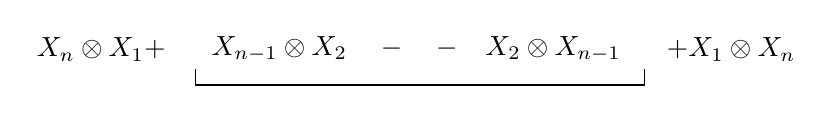
\begin{tikzpicture}
\node (a) at (0,0) {$X_n\otimes X_1+$};
\node (b) at (4.0,0) {$X_{n-1}\otimes X_2\quad-\quad-\quad X_2\otimes X_{n-1}$};
\node (c) at (8.0,0) {$+X_1\otimes X_n$};
\draw (1.2,-.25)--(1.2,-.45)--(6.9,-.45)--(6.9,-.25);
\end{tikzpicture}}
\[\unsure{U_n|\mathcal U_n|U_m|\mathcal U_m}\qquad\delta X_n\]
% Lower-right abandoned arrows, then live diagram.
\diagram{\begin{tikzcd}[ampersand replacement=\&]
\deleted{\unsure{\delta}}\&\deleted{U}\arrow[r]\&\deleted{U\otimes U}\arrow[r]\&\deleted{U}
\end{tikzcd}}
\diagram{\begin{tikzcd}[ampersand replacement=\&]
A\&A\otimes A\arrow[l]\&A\arrow[l]\\
G\arrow[r,"{\text{diag}}"']\&G\times G\arrow[r,"{\text{mult.}}"']\&G
\end{tikzcd}}
% Lower-left computation and continuation to its right.
\[X_2\]
\[X_1^2=2X_2+X_1\]
\[
\left\{\begin{aligned}
2X_2&=X_1^2-X_1\\
\delta X_2&=X_1\otimes X_1
\end{aligned}\right.
\qquad ?\qquad 2\delta X_2=\delta(X_1^2-X_1)
\]
\[\deleted{\unsure{2.\delta(X_1}}\]
\[2X_1\otimes X_1=\delta(X_1^2-X_1)\]
\[
\begin{aligned}
\delta(X_1)&=X_1\otimes1+1\otimes X_1\\
\delta(X_1^2)&=X_1^2\otimes1\unsure{-|+}1\otimes X_1^2+2X_1\otimes X_1
\end{aligned}
\]
\scanpage{31}
% archive sheet number: 30
% Typescript is upside down in the supplied scan; transcribed in its reading direction.
\mspage{21}
n\textsuperscript{o} 246

% Printed lines 1--6.
donc, en vertu de la relation (14), $x_{\handwritten{31}}\handwritten{<}0$, donc ($\unsure{\Delta|\handwritten{\Delta}}_{\handwritten{0}},\Delta_{\handwritten{1}},\Delta_{\handwritten{3}}$) est directe. Soit donc $x_{\handwritten{01}}\handwritten{>}0$ ; si $x_{\handwritten{30}}\handwritten{<}0$, on a $x_{\handwritten{02}}\handwritten{>}0$, $x_{\handwritten{23}}\handwritten{>}0$ (parce que la seconde suite est directe), puis $x_{\handwritten{12}}\handwritten{>}0$ (parce que la première est directe), d'où $x_{\handwritten{13}}\handwritten{>}0$, d'après (14), et ($\Delta_{\handwritten{0}},\Delta_{\handwritten{1}},\Delta_{\handwritten{3}},$) est directe. Il en est de même, enfin, si $x_{\handwritten{01}}\handwritten{>}0$, $x_{\handwritten{30}}\handwritten{>}0$. les autres axiomes de la relation d'ordre se vérifient trivialement.

% Printed lines 7--10; underlining does not continue beneath the formula blanks.
Corollaire. - \uline{Soient} $\Delta_i$ ($0\handwritten{\leq}i\handwritten{\leq3}$) \uline{quatre demi-droites telles que la suite} $\Delta_{\handwritten{0}},\Delta_{\handwritten{1}},\Delta_{\handwritten{2}}$ \uline{soit directe}. \uline{Alors}, \uline{pour que la suite} $\Delta_{\handwritten{1}},\Delta_{\handwritten{3}},\Delta_{\handwritten{2}}$ \uline{soit directe}, \uline{il faut et il suffit que les deux suites} $\Delta_{\handwritten{0}},\Delta_{\handwritten{1}},\Delta_{\handwritten{3}}$ \uline{et} $\Delta_{\handwritten{0}},\Delta_{\handwritten{3}},\Delta_{\handwritten{2}}$ \uline{le soient}.

% Printed lines 11--16.
Pour abréger, notons (ijk) l'assertion ``\unsure{lasuite|la suite} $\Delta_i,\Delta_j,\Delta_k$ est directe''. D'après la prop. 6 (132) et (120) entraîne (130) ; et (201) et (213) entraîne (203) ; donc le condition du corollaire est nécessaire. Réciproquement, supposons (012), (013) et (032) vérifiées ; si (123) était vérifiée, alors on aurait (310), car (312) et (320) entraîne (310) d'après la prop. 6. Cette contradiction achève la démonstration.

% Printed lines 17--26; final sentence continues beyond the sheet.
Si $\Delta_{\handwritten{1}},\Delta_{\handwritten{2}}$ sont deux demi-droites distinctes, on voit immédiatement (en prenant une base formée d'un vecteur de $\Delta_{\handwritten{1}}$ et d'un vecteur de $\Delta_{\handwritten{2}}$) qu'il existe une demi-droite $\Delta_{\handwritten{0}}$ telle que la suite $\Delta_{\handwritten{0}},\Delta_{\handwritten{1}},\Delta_{\handwritten{2}}$ soit directe. Il résulte alors de la prop. 6 et de son corollaire que, pour la relation d'ordre déterminée par $\Delta_{\handwritten{0}}$ comme dans la prop. 6, les intervalles ouvert et fermé $\handwritten{]}\Delta_{\handwritten{1}},\Delta_{\handwritten{2}}\handwritten{[}$ et $\handwritten{[}\Delta_{\handwritten{1}},\Delta_{\handwritten{2}}\handwritten{]}$ sont indépendants du choix de $\Delta_{\handwritten{0}}$. La réunion des demi-droites d'un tel intervalle s'appelle un \uline{secteur angulaire}. Autrement dit, on appellera \uline{secteur angulaire ouvert} $\handwritten{]}\Delta_{\handwritten{1}},\Delta_{\handwritten{2}}\handwritten{[}$ la réunion des demi-droites $\Delta$ telles que la suite $\Delta_{\handwritten{1}},\Delta,\Delta_{\handwritten{2}}$ soit directe, et \uline{secteur angulaire fermé} $\handwritten{[}\Delta_{\handwritten{1}},\Delta_{\handwritten{2}}\handwritten{]}$
\scanpage{32}
% archive sheet number: 31
% Landscape sheet; faint mirrored typescript is verso show-through.
% Upper-left and upper-right formulas.
\[
X_n(t^m)=\binom mn t^m\qquad\langle X_n,t^m\rangle=\binom mn
\]
\[X_nX_{n'}(t^m)=\binom mn\binom m{n'}\]
\margin{nul si}
\[\deleted{\unsure{X_n,\,s+t^c|X_n,\,s+c}}\]
\[t=1+s\unsure{\Rightarrow|=}\ ,\quad s=t-1\]
\[
\frac{m(m-1)\;--\;(m-n+1)}{n!}\ \frac{m(m-1)\;--\;(m-n'+1)}{n'!}
\]
% Isolated trial symbols on left.
\[\deleted{\unsure{n|m}}\qquad\Delta X_n\]
\[\mbox{\Large$X$}\qquad\Delta X_{\unsure{-|n}}\]
\figure{\begin{tikzpicture}
\draw (0,1.2)..controls(-.35,1.18)and(.25,1.05)..(0,1.0)..controls(-.2,.94)and(.2,.86)..(0,.79)..controls(-.18,.72)and(.18,.64)..(0,.58)..controls(-.12,.48)and(.2,.32)..(.08,0);
\end{tikzpicture}}
% Upper-right binomial expansion, with the handwritten dashes retained.
\[
\begin{aligned}
\langle X_{\unsure{m|n}},s^m\rangle&=\langle X_n,(t-1)^m\rangle\\
&=\binom mn-\binom m1\binom{m-1}n+\binom m2\binom{m-2}n\\
&\qquad-\qquad+(-1)^k\binom mk\binom{m-k}n+\;-
\end{aligned}
\]
\[+\]
% Central computation.
\[
\langle X_{\unsure{1|b}}(t-1)^m\rangle=\left.tm(t-1)^{m-1}\right|_{t=\unsure{1|4}}
=\left\{\begin{aligned}
0&\quad\text{si }m\unsure{\ne|=}1\\
1&\quad\text{sinon}
\end{aligned}\right.
\]
\[
\deleted{\unsure{\langle|\Delta}}\langle X_2,(t-1)^m\rangle=\left\langle\frac{X_1^2}{2}-\frac{X_1}{2}\right\rangle
\]
\[\boxed{\unsure{t-1|t-1^5}}\qquad\frac{m(m-1)}{2!}-m\ .\]
\[\deleted{X_n,s^m}\]
\[X_2(t-1)=X_2(t)=\binom12\]
% Lower-left marginal identity.
\margin{$X_n=\binom Xn$}
\[
\underset{m\geq0}{X_n(t^m)}=\left\{\begin{aligned}
0&\quad\text{si }m<n\\
t^n&\quad\text{si }m=n\\
-&
\end{aligned}\right.
\]
% Lower-right unfinished cases and isolated power.
\[
X_n((t-1)^m)=\left\{\begin{aligned}
0&\quad\text{si }\underline{0\leq m<n}\\
t^{\unsure{n|m}}&\quad\text{si }m=n\\
0&\quad\text{si }\ .
\end{aligned}\right.
\qquad(t-1)^r
\]
\[\langle X_n,s_{\deleted{\unsure{m}}}^{m}\rangle=\delta_{nm}\qquad\unsure{\langle|\{}X_n,s^m\rangle\]
